\chapter{Gaussian Processes - Rasmussen}

\begin{defn}
    For any set $S$, a \newterm{Gaussian process} (GP) on S is a set of random variables ($Z_t : t \in S)$ such that $\forall n \in \sN, \forall t_1, \dots, t_n \in S$ the random vector $(Z_{t_1}, \dots, Z_{t_n})$ is a Gaussian.
\end{defn}

\begin{thm}[Existence of Gaussian Processes]
    For any set $S$, any mean fn $\mu : S \rightarrow \sR$, and any covariance fn $k : S \times S \rightarrow \sR$, there exists a GP $(Z_t)$ on $S$ such that $E Z_t = \mu(t), cov(Z_s, Z_t) = k(s, t), \forall s,t \in S$.
\end{thm}

Note: It is enough to specify the pairwise covariances and don't need to define it on every subset. This is a special property of Gaussian properties, and does not hold for a general stochastic process. \todo{proof?}

\section{Posterior}

A GP defines a prior distribution over functions. 

\begin{equation}
    \begin{pmatrix}\vf \\ \vf_*\end{pmatrix} \sim \gN \left(\mZero, \begin{pmatrix}\mK & \mK_* \\ \mK^T_* & \mK_{**} \end{pmatrix} \right)
\end{equation}

Using the theorem {TODO marginal conditional ref} we can directly compute the posterior parameters

\begin{align}
    \mu_* &= \mK_*^T \mK_*^{-1} y \\
    \Sigma_* &= \mK_{**} - \mK_*^T \mK_*^{-1} \mK_*.
\end{align}


\section{Kernels}

Examples of Gaussian Processes:

\begin{itemize}
    \item Random lines, $S = \mR, Z_t = t \mW, \mW \sim N(0, 1)$ by the affine property.
    \item Random planes: $S = \mR^d, \mu(x) = 0, k(x,y) = x^T y$.
    \item Std. Brownian Motion: $S = [0, \infty), \mu(t) = 0, k(s, t) = min(s, t)$. (also somehow includes that it is continuous with $P = 1$).
    \item Squared exp: $S = \mR, \mu(x) = 0, k(x,y) = e^{-\alpha ||x - y||^2}, \alpha > 0$ (should be infinitely differentiable with $P = 1$) (Gaussian kernel, in 2D it is called Gaussian random field {TODO vygooglit}).
    \item Orenstein-Uhlenbeck: $S = [0, \infty), \mu(t) = 0, k(s, t) = e^{-\alpha |s - t|}, \alpha > 0$ (Laplace kernel).
    \item A periodic GP: $S = \mR, \mu(t) = 0, k(x, y) = e^{-\alpha \sin(\beta\pi(x - y))^2}, \alpha, \beta > 0$.
    \item A Symmetric GP: $S = \mR, \mu(t) = 0, k(x, y) = e^{-\alpha min(|x-y|, |x+y|)^2}, \alpha>0$.
\end{itemize}

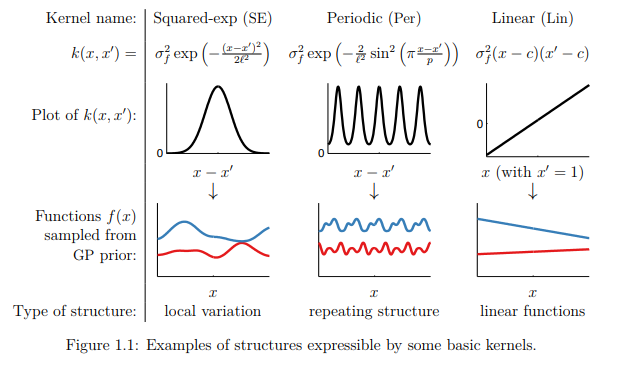
\includegraphics[width=0.7\textwidth]{img/kernels}

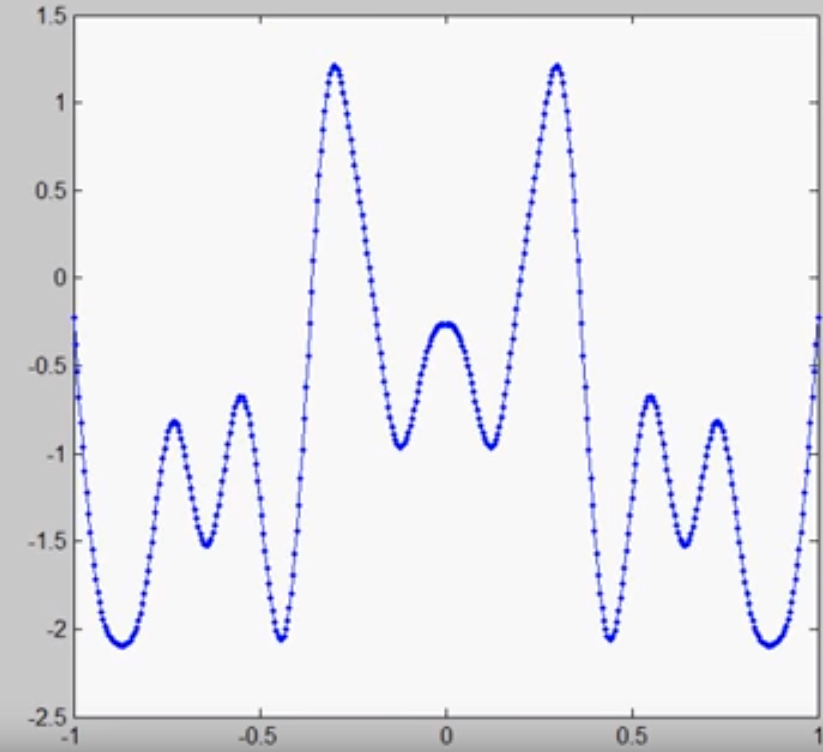
\includegraphics[width=0.7\textwidth]{img/symmetric-kernel}

Image stolen from https://www.cs.toronto.edu/~duvenaud/cookbook/

\section{Kernel Hyperparameters}

TODO


\begin{tcolorbox}
    \newterm{Gaussian Process} is a \newterm{stochastic process} (a collection of random variables), such that every subset of those random variables has a multivariate Gaussian distribution. It is defined by a mean function $m(x)$ and a covariance funciton $\kappa(x, x')$. Formally, we write {TODO osklive GP}:
    
    \begin{equation}
    f(x) \sim \gN \gG \gP (m(x), \kappa(x, x'))
    \end{equation} {TODO finish}
    
    Bayesian inference ...
    
    \begin{equation}
        \text{posterior} = \frac{\text{likelihood} \times \text{prior}}{\text{evidence}}
    \end{equation},
    
    where evidence is also called \newterm{marginal likelihood}. More concretely, we usually want to compute the posterior distribution over the parameters $\vw$ given the inputs $\mX$ and outputs $\vy$
    
    \begin{equation}
        p(\vw | \vy, \mX) = \frac{p(\vy | \vw, \mX) p(\vw)}{p(\vy | \mX)}
    \end{equation}.
    
    The marginal likelihood is independent of the weights and acts as a normalizing constant. We compute it using marginalization
    
    \begin{equation}
        p(\vy | \mX) = \int p(\vy | \vw, \mX) p(\vw) d \vw.
    \end{equation}
    
    {TODO describe prior over functions}
\end{tcolorbox}

Note: GP regression and Bayesian Linear Regression are equivalent except for the kernel vs basis functions.

\begin{itemize}
    \item Bayesian Lin. Reg: $D = ((x_1, y_1), \dots, (x_n, y_n)), x_i \in \mR^d, y_i \in \mR$
    
    $Y_1, \dots, Y_n$ independent given $w$
    
    $p(y_i | x_i, w) = N(y_i | \vw^t x_i, \sigma^2)$, i.e. $Y_i = w^T x_i + \epsilon_i$.
    
    $w \sim N(0, v\mI) \implies \forall x \in \mR^d, w^t x$ is a univariate Gaussian {TODO thanks to our magic definition lol}
    
    $Z_x = x^t w$ is a GP on $S = \mR^d$.
    
    Let $x_1, \dots, x_n \in \mR^d$ and we need to show that $(Z_{x_1}, \dots, Z_{x_n})^T$ is a multivariate Gaussian.
    
    $(Z_{x_1}, \dots, Z_{x_n})^T = (x^T_1 w, \dots, x^T_n w)^T = (x^T_1, \dots, x^T_n)^T w = X w$, and since $w$ is a Gaussian, by the affine property we know $X w$ is also a Gaussian.
    
    $\mu(x) = E Z_x = E x^t w = x^t E w = 0$
    
    $cov(w) = E w w^t - \underbrace{E w E w^t}_0 = v \mI$
    
    \begin{align}
        k(x, x') &= cov(Z_x, Z_x') = E Z_x Z_x' - \underbrace{E Z_x E Z_x'}_0 \\
        &= E x^t w w^T x' \quad \text{quadratic form in } w w^T \\
        &= x^t E[w w^T] x' \\
        &= x^t v \mI x' = v x^t x' \quad \text{this is the plane GP}
    \end{align}
\end{itemize}

\section{GP from scratch again}

Let $Z \sim N(\mu, K), \epsilon \sim N(0, \sigma^2 \mI)$ independent. Let $Y = Z + \epsilon$, then $Y \sim N(\mu, K + \sigma^2 \mI)$. {TODO ref earlier theorem}.

TODO

\section{Decision theory for GP regression}

Our goal is to make a point prediction $y_\text{guess}$ which incurs the smallest loss without knowing $y_\text{true}$. We minimize the $expected loss$ {TODO use proper term} by averaging w.r.t. our model's posterior.

\begin{equation}
    \hat R(y_\text{guess} | x_s ) = \int \gL (y_s, y_\text{guess} p(y_s | x_s, D) \d y_s.
\end{equation}

\begin{equation}
    y_\text{optimal} | x_s = argmin_{y_\text{guess}} \hat R_\gL(y_\text{guess} | x_s).
\end{equation}

The selection of a covariance function and finding its parameters is referred to as \emph{training} the GP.



\section{Noise-less Gaussian Process Regression}

\section{Noisy Gaussian Process Regression}


